\documentclass[conference]{IEEEtran}
\IEEEoverridecommandlockouts
% The preceding line is only needed to identify funding in the first footnote. If that is unneeded, please comment it out.
\usepackage{cite}
\usepackage{amsmath,amssymb,amsfonts}
\usepackage{algorithmic}
\usepackage{graphicx}
\usepackage{textcomp}
\usepackage{xcolor}
\usepackage{subcaption}
\usepackage{graphicx}
\def\BibTeX{{\rm B\kern-.05em{\sc i\kern-.025em b}\kern-.08em
    T\kern-.1667em\lower.7ex\hbox{E}\kern-.125emX}}
\begin{document}

\title{Deep Reinforcement Learning-Based Energy Trading of Microgrid with Mitigating the risk of disturbances 
\thanks{This is for the final report in ME 597: Distributed Energy Resources - Spring 2024 }
}

\author{\IEEEauthorblockN{1\textsuperscript{st} Jae Heo}
\IEEEauthorblockA{\textit{School of Construction Management Technology} \\
\textit{Purdue University}\\
West Lafayette, IN, USA, 47906 \\
heo27@purdue.edu}

}

\maketitle

\begin{abstract}
The occurrence of large-scale disturbances has been increasing over 20 years in the United States. As a consequence of this trend, a primary concern of today's power system is to enhance its resilience. As an innovative solution, microgrids suggest an immense promising approach toward achieving a higher level of distribution system resilience by integrating with electricity load. Although previous studies have 
\end{abstract}

\begin{IEEEkeywords}
Microgrid, Resilience, Large disturbance, Energy trading, Deep reinforcement learning
\end{IEEEkeywords}

\section{Introduction}
The escalating frequency and intensity of extreme weather events pose significant threats to energy infrastructures, with the electrical power system being particularly vulnerable to disruptions and consequent substantial losses. Natural hazards, such as earthquake and severe storms, annually cause considerable damage to the electric power sector, exemplified by data from the National Centers for Environmental Information. Since 1980, the U.S. averaged annually 6.7 weather-related disasters resulting in losses exceeding \$1 billion across three consecutive decades. This increasing trend in natural disasters, especially those related to heat, is alarmingly attributed to anthropogenic climate change, heightening the urgency for effective research into mitigation strategies. 

Distributed generation is an alternative to familiar centralized generation as it is the central concept is decreasing the distance between generation and consumption areas. This in turn can decrease the high transmission costs and potential losses which Sudan suffers greatly from at approximately 25 \% transmission loss. Microgrids are a type of smart grids that represent the smallest type of distributed network. They are a collection of generation/consumption units that exist in a small area. Microgrids are generally used to power a small village, island or a confined residential area. Microgrids use distributed-renewable energy sources as the generation, increasing the usability of them for the new area.

As regards power system resilience, the emergence and development of a broad array of smart grid technologies, architectures, and applications offer viable, intelligent solutions. Toward this end, microgrid (MG), an essential part of smart grids, could afford unprecedented opportunities. Briefly speaking, MGs are small-scale power systems connected to the distribution system (DS) at the low- or medium-voltage level, capable of integrating distributed energy resources (DERs) and being operated in stand-alone or grid-tied modes. Owing to these capabilities, MGs have shown great potential to improve system resilience. In recent years there has been an increasing amount of literature emphasizing the optimal use of DERs and MGs in improving power system resilience. The optimal MG energy management and control are significant contributors to realizing its potential, especially in achieving higher levels of resilience. Optimal energy management of MGs entails minimum operation cost and maximum supply coverage while coordinating the tasks of dispatchable and non-dispatchable DGs, ESSs, adjustable loads, and remote-controlled switches under all conditions. Therefore, different aspects of the optimization problems have to be fully considered. In this regard, accurate modeling of MG components and proper capture of the uncertainties play a significant role. The prevalent constraints to be considered are dispatchable generation capacity, distribution lines thermal limit, voltage and current limits, state of charge and capacity of batteries, as well as frequency fluctuation limits which must be controlled by at least one generation resource within each MG. However, inherent uncertainties associated with the optimal operation of MGs lead power system researchers to use stochastic models.

\section{Literature Review}
With the deployment of the smart grid, and especially the ever-increasing penetration of DERs and remotely controllable switch devices, intentional and controlled islanding from RESs and dispatchable DGs is regarded as a promising approach to enhance the DS resilience against major events. A potential solution to achieve this goal is to well exploit these resources and switches by intentionally splitting the DS into multiple self-supplied MGs. As stated in the IEEE standard 1547.4 [64], dividing the DS into several MGs can improve the system’s operation and reliability.

The logic behind electric service restoration through optimal MG formation is to optimally allocate resources to maximize the total weighted sum of restored loads by locally supplying them through DERs until the complete restoration of the main grid. To do so, the optimal switching plan must be conducted; if there is a lack of controllable switches, this plan will equal an optimal placement problem of sectionalizing switches.

From a practical standpoint, following a major event occurrence—assuming that the communication and monitoring system is reliable—the network configuration and system failures would be specified. After isolating the least portion of the network containing faulted zone by controllable switches, the self-healing system reconfiguration will partition the network into an optimal number of self-adequate MGs to serve loads locally [65]. However, some challenges exist in efficiently forming MGs from several RESs and DGs, especially in the case of facility destructions or communication system collapse [66].

\subsection{Uncertainty Capture}
aspect in modeling MG formation within the DS is whether to consider the uncertainties (mentioned in Subsection II-C) or not, which will result in stochastic/robust or, more frequently, deterministic problems, respectively. In a notable paper, Wang and Wang [73] develop a double-stage stochastic optimal DS operating framework as an MINLP problem comprising normal and self-healing modes. In the case of a fault or multiple faults, the system enters the self-healing mode by optimally transforming the on-outage portion of the distribution network into networked, self-adequate MGs to re-energize as much as possible loads. The uncertainties in load and non-dispatchable generation are considered by a normal distribution and stochastic rolling horizon optimization concept, respectively.

Considering the supply-demand uncertainties, Popovic et al. [74] model MG formation as a minimax problem while minimizing the risk of unsuccessful islanding due to unmet local load. Taking into account the same uncertainties, Sharma et al. [75] develop a decentralized MAS to form self-sufficient islands with DERs. In another article, Biswas et al. [76] adopt a chance-constrained approach to model the probabilistic, optimal DS sectionalizing problem while capturing the demand-supply uncertainties.

\subsection{Mitigation of risk of disturbance in the Microgrid}
While most papers seek to form self-sufficient MGs within the DS, some research works model and investigate the power exchange among formed MGs or even the formation of NMGs. Adopting a graph-theoretical approach, Arefifar et al. [98] propose an optimal DERs allocation and MG formation framework while studying energy transfer effects among formed MGs. Ding et al. [99] develop a MILP model to co-optimize the RC routing and repair time, routing and charging strategy for MESSs, and network reconfiguration leading to the formation of Soft-Open-Point (SOP)-based NMGs ([100] and [101] provide a systematic review of emerging SOP technology in DSs). Barani et al. [102] suggest a two-stage model for optimal placement of DERs and protection devices and subsequent DS partitioning into multiple MGs while considering power exchange among them.

Power system communication is the Achilles heel of the system during the restoration process, and a lack of resilient communication infrastructure would jeopardize situational awareness. There are several published studies describing the role and requirements of the communication system in enhancing resilience ([111], [112], [113], to cite a few). However, some studies incorporate communication resilience in the optimal MG formation problem. Chen et al. [66] propose a MILP model for radial DS restoration strategy by forming multiple self-supplied MGs. This model fulfills communication resilience requirements by designing a distributed multi-agent coordination scheme. To reduce the computational complexity of this model, Ding et al. [114] reformulate the model proposed in [66] by lessening the scale of binary variables. To comply with the requirement of real-time status communication in the case of large-scale disturbances, Qi et al. [115] suggest a new system design including the embedment of intelligent power electronic devices and control schemes. This scheme realizes a reconfigurable system and intentional islanding of a MG or a portion of the power grid.

\section{Data Generation}
This project uses four types of energy data (5-minute resolutions) on potential electricity by Solar power, electricity loads, electricity price, the risk of disturbance in solar power plants, and in load, which are known to significantly affect energy trading in microgrids. Unfortunately, we could not collect relevant datasets in real ones, and thus we generated all data by utilizing mathematical formulation (the risk of disturbance), class material (solar energy, electricity load), and statistics(electricity price). 
First, the risk of disturbance in PV and load could be generated depending on the recent national renewable energy laboratory research \cite{b1}. It provides a new statistical methodology that calculates the impact of distributed energy reliability and variability on a microgrid`s performance for the risk of disturbance in PV. They demonstrated that a utility-scale PV system's availability is typically greater than 99\% and the capacity may decline on the order of 1\%. Accordingly, we assumed that the probability risk of disturbance in PV is 1\% and its probability is equal to the probability risk of disturbance in load. Second, solar energy and electricity load can be computed by using class material that is der-solar and der-buildings. lastly, we assumed that the electricity price is constant unlike Indiana state, but fluctuates like the European Union involves volatility in peak load. Overall, the electricity load and solar power output including the risk of disturbance ranges from 0 to 19.0 (kW) in generation and 0 to 2.3 (kW) in consumption. Specifically, when an emergency situation happens in the generation or consumption stage, the electricity values are dropped to 0. 
\begin{figure}[htbp]
    \centering
    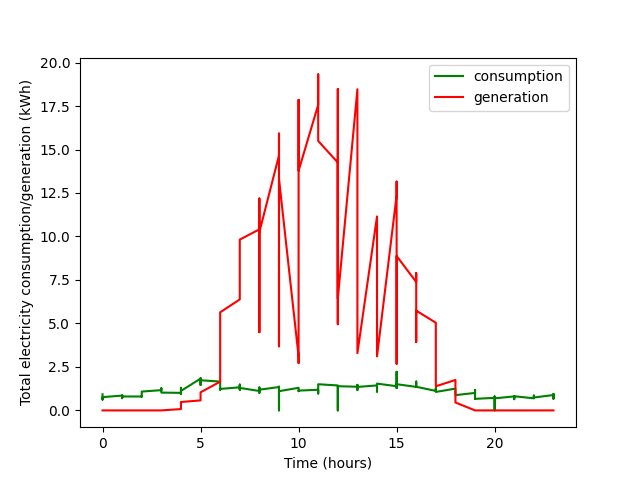
\includegraphics[width=0.5\textwidth]{report/figure/data_collection_1_v1.png}
    \caption{The electricity generation and consumption with the risk of disturbance.}
    \label{fig:1}
\end{figure}

\section{Reinforcement learning}
The mathematical context of Markov decision process (MDP) can be considered as a formal framework to formalize diverse RL methods for learning optimum decision-making policies in a fully or partially observable environment. One of the important issues is the intelligent agent can dynamically make decisions based on actions, states, and rewards where the states refer to possible network configurations and reward (or penalty) stands for feedback signal from the network (environment) that implies the agent’s performance. However, traditional RL has distinct two limitations: (1) Difficulty of applicability to the complex environment and (2) Dendepent on the single agent problem. Traditional RL cannot perform well in the complex environment when the agent encounters the state for the first time. This is because MDP-based traditional RL should control and compute the probability of all states within the environment. Moreover, traditional RL only explores the single agent for the simplicity of the model. They only solved the common problem that all agents take the same actions sharing states. However, most of the world does not have the same characteristics in the agents corresponding to a state. Overall, recent researchers have solved this problem by using deep neural network and multi-agent concepts. 

\subsection{A2C MARL}
To overcome these challenges in traditional DRL, recent studies have employed the actor-critic method with a baseline $b_t$, which compares the cumulative reward in the policy gradient as expressed by \textbf{Equation \eqref{eq_4}}
\begin{equation} \label{eq_4}
    J(\theta) = \mathbb{E}[\sum_{0}^{T-1}\nabla_{\theta}\log(a_t|s_t)(G_t-b(s_t))], G_t = \sum_{t'=0}^{T-1}\gamma^{t'}R_{t'}
\end{equation}
The actor-critic is a hybrid architecture combining a policy-based method in the actor, which controls how the agent behaves, and a value-based method in the critic, which estimates what the best action taken by the Actor is. In the actor-critic method, the policy gradient ($J(\theta)$, actor loss) is represented by the subtraction of cumulative reward with a baseline ($G_t - b(s_t)$) in \textbf{Equation \eqref{eq_4}}. From the Bellman optimal equation, \textbf{Equation \eqref{eq_4}} can be rewritten as the advantage function ($A_t$), which compares taking specific action to the average action at the given state using the Q value and V value, as shown in \textbf{Equation \eqref{eq_5}}. 
\begin{equation} \label{eq_5}
    \nabla_{\theta} J(\theta) =\sum_{0}^{T-1}\nabla_{\theta}\log\pi_\theta(a_t|s_t)A_t , A_t = r_{t+1} + \gamma V_{\phi}(s_{t+1}) - V_{\phi}(s_t)
\end{equation}

Moreover, the A2C is approximated toward minimizing the loss $L(\theta)$, which is a combination of Actor and Critic losses for optimizing the model. Actor loss is calculated by policy gradient and the critic losee estimates the expected returns ($G_t$) for q-values using the mean squared error (i.e., squared L2 norm) expressed by \textbf{Equation \eqref{eq_6}}
\begin{equation} \label{eq_6}
    L_{critic} = (\sum_{t'=0}^{T-1}\gamma^{t'}r_{t'}-V_\phi(s_t))^2
\end{equation}

In contrast to typical deep learning approaches where the loss function compares predictions with ground truth values using error metrics (e.g., L1 loss, L2 loss) in deep learning, the loss function in the DRL optimizes not the reward function directly but the product of the estimated value function and the probability of the action. 

The critic loss represents the estimation of the value of the state to minimize the temporal difference (TD) error, which is the difference between $s_t$ and $s_{t+1}$, using gradient descent \textbf{Equation \eqref{eq_9}}

\begin{equation} \label{eq_9}
    \phi = \phi + \alpha\delta\nabla_{\phi} V_{\phi}(s)
\end{equation}

where $w$ denotes the set of parameters of the value function (critic network), $\alpha$ denotes the learning rate, $\delta$ denotes the TD error, and $\nabla_w V(s,w)$ denotes the gradient of the critic network.

Also, the actor loss determines the probability of the action selected by $\pi_{\theta}(a|s)$, as expressed by \textbf{Equation \eqref{eq_10}}

\begin{equation} \label{eq_10}
    \theta = \theta + \alpha\delta\nabla_{\theta}\log\pi_{\theta}(a|s)
\end{equation}

where $\theta$ denotes the set of parameters of the actor network, and $\nabla_{\theta}\log\pi_{\theta}(a|s)$ denotes the probability of selecting action $a$ by policy $\pi_{\theta}$. 

\subsection{Algorithm}
Multi-agents represent the prosumer, an individual who is both consumes and produces, producer, and consumer. They take three actions the role of battery, and pairs of emergency responses (generation, consumption). The role of the battery ($a_1$) includes that trading the surpluses and shortages of electricity with an external network, charging batteries by the surplus of electricity production, discharging the battery when consumption is greater than production to compensate required energy. In more detail, to take action of the role of battery among three action probabilities, Firstly, we computed the current battery state (CBS) using \textbf{Eq. \eqref{eq_111}}
\begin{equation} \label{eq_111}
    CBS = PBS + (a_1 - 3 ) * (a_1 - 4) * Surp
\end{equation}
where PBS is previous battery state and Surp denotes the surplus electricity. Furthermore, through three actions, we calculate the reward function with seven reward factors: reward for charging the battery, reward for charging the battery with selling the surplus energy, reward for discharging the battery, reward for selling the surplus energy with selling price, reward for buying energy from the grid, reward for the emergency responded in PV, and reward for the emergency responded in load. For example, in the reward for charging the battery, when the agent charges the battery too much, we give the penalty to prevent the charging values over battery capacity. Overall, the reward function can be computed by summing these reward factors.
Finally, carbon dioxide (CO$_2$) emission can be computed by multiplying surplus energy with 03855535 (conversion of energy shortfall (kWh) into emitted CO$_2$ (kg). 

\section{Result}
This project tested the developed algorithm with re-implementing the algorithm (\cite{b4}) to detect the risk of disturbances in generation and consumption and to mitigate this emergence in the energy training on the microgrid concept. \textbf{Fig. \ref{fig2} and \ref{fig3}} displayed the convergence curves of the 1000-episode moving of the episodic total reward in the distribution network for the two different MARL algorithms. 
\begin{figure}[htp]
\begin{subfigure}{0.45\columnwidth}
  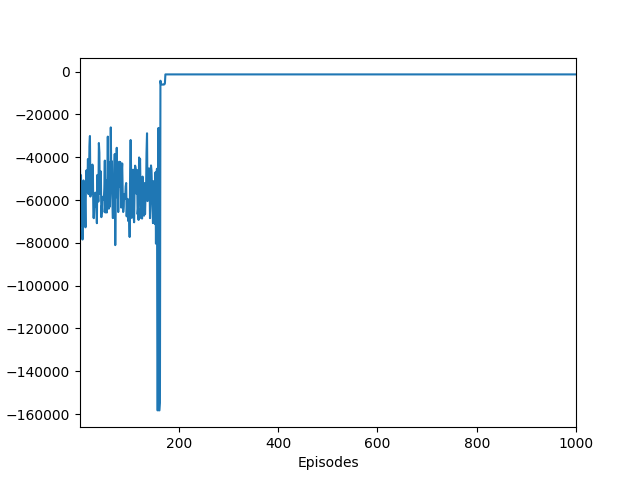
\includegraphics[width=\textwidth]{report/figure/result_1_v1.png}
  \caption{Learning graph via reward in first agent}
  \label{fig2}
\end{subfigure}
\hfill
\begin{subfigure}{0.45\columnwidth}
  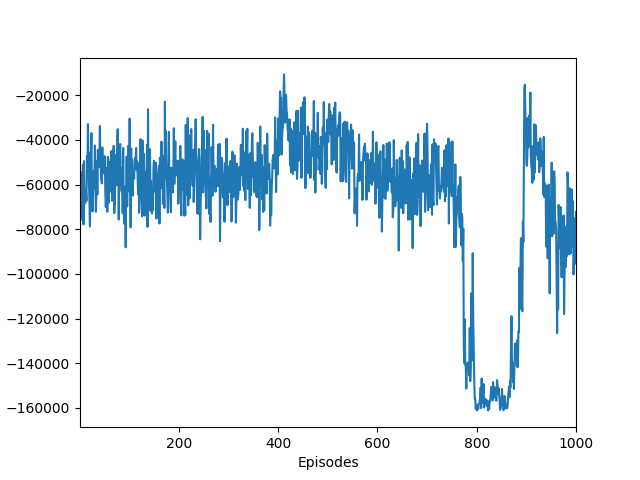
\includegraphics[width=\textwidth]{report/figure/result_1_v2.png}
  \caption{Learning graph via reward in second agent}
  \label{fig3}
\end{subfigure}
\end{figure}
It is evident that the first agent's episodic total reward can be converged in around 200 episodes. On the other hand, the second agent's episodic total reward cannot be converged in whole episodes, in addition, to the catastrophic problem after around 800 episodes. It implies that the learning model abruptly forgets previously learned information upon learning new information and falls into the local minima solution. 

Additionally, \textbf{Fig. \ref{fig4} and \ref{fig5}} shows the evaluation of detection success whether the model can take correct actions (emergency response) corresponding to the ground truth (actual emergence class: 1. night, 2. daytime, 3. peak time, 4. emergency). 
\begin{figure}[htp]
\begin{subfigure}{0.45\columnwidth}
  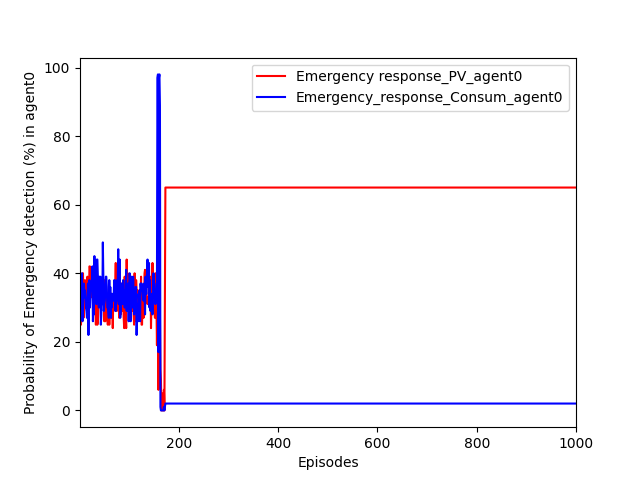
\includegraphics[width=\textwidth]{report/figure/result_2_v1.png}
  \caption{The evaluation of detection success for PV and load in first agent}
  \label{fig4}
\end{subfigure}
\hfill
\begin{subfigure}{0.45\columnwidth}
  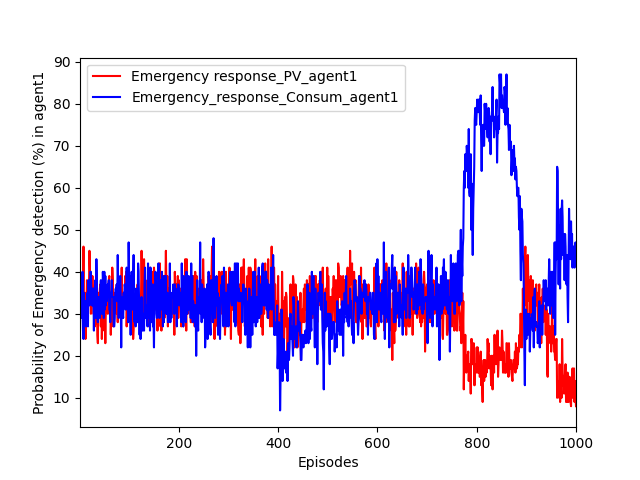
\includegraphics[width=\textwidth]{report/figure/result_2_v2.png}
  \caption{The evaluation of detection success for PV and load in second agent}
  \label{fig5}
\end{subfigure}
\end{figure}
The red lines represent the accuracy of detection success for PV in first agent and second agent and the blue lines represent the accuracy of detection success for load in first agent and second agent. The results showed that the two agents got similar accuracy about around 40\% until the convergence in first agent and catastrophic problem in second agent. Specifically, the first agent has distinct patterns after convergence points that the accuracy of emergency response in PV is higher than in consumption. On the other hand, the second agent has opposite patterns with first agent that the accuracy of emergency response in consumption is higher than in generation. It implies that there are subsequent relationship between generation and consumption in emergency response. 

To further analysis of our model, we showed how the model can mitigate load disturbance in energy trading. it is represented by battery capacity (kW). Both of results \textbf{Fig. \ref{fig6} and \ref{fig7}}showed that the mitigation of energy trading occurs in the load disturbance.

\begin{figure}[htp]
\begin{subfigure}{0.45\columnwidth}
  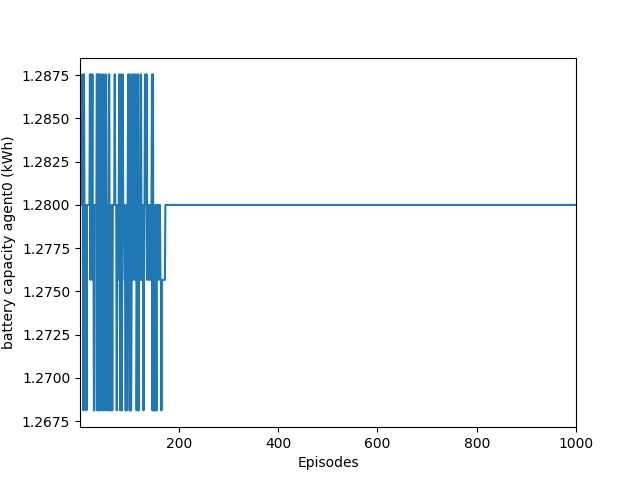
\includegraphics[width=\textwidth]{report/figure/result_3_v1_2.png}
  \caption{The mitigation of emergency situation on the energy trading (battery capacity) in first agent}
  \label{fig6}
\end{subfigure}
\hfill
\begin{subfigure}{0.45\columnwidth}
  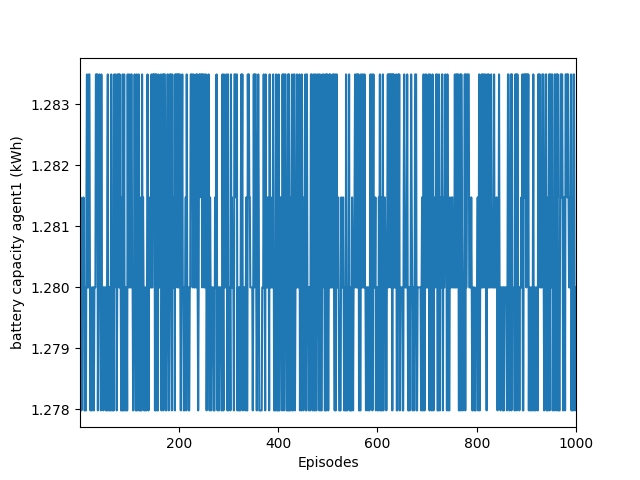
\includegraphics[width=\textwidth]{report/figure/result_3_v2.png}
  \caption{The mitigation of emergency situation on the energy trading (battery capacity) in second agent}
  \label{fig7}
\end{subfigure}
\end{figure}

The results showed that the range of battery capacity can be formed 1.2675 (kW) to 1.2875 (kW) in the first agent until convergence points and 1.278 (kW) to 1.283 (kW) in the second agent until the catastrophic problem. The reason for the tiny gap between maximum and minimum capacity may be related with the data time resolution. Our data time resolution is 5 minutes that cannot be substantial consumption or generation between 5-minute laps. These ranges are dramatically reduced in the occurrence of emergency situations. It implies that the model can sufficiently mitigate the dramatic energy changes by emergency disturbances and have a stable learning with mitigation. This stable pattern disappears after convergence in the first agent and the catastrophic problem in the section agent. 

Finally, the reduction of CO$_2$ emissions through surplus electricity is a constant as 0.1243 (kg).

\section{Discussion \& Conclusion}
This project developed the microgrid energy trading model with mitigating emergency disturbance using deep reinforcement learning. Proposed method tried to detect the emergency events while estimating the energy trading with maximizing the reduction of CO$_2$ emissions. However, the proposed method can stably learn the energy trading rule well but has low performance in detecting emergency situation. There are two reasons (1) low quality of datasets and (2) deficiency of extracting features in the environment. One of reason for this problem may be caused by the low quality of the dataset. We split one dataset, computed by one simulation, into two sets for two agents. Two agents shared similar information patterns and it may result in poor learning performance. Moreover, our model built up with a deep neural network (i.e., a fully connected model) cannot capture sufficient features on the numerical state from the dataset. General DER or Microgrid datasets are graph-structured format that involves the relationship between agents, and energy trading networks with hidden features. However, time series-based table-shaped datasets did not include this relationship and network features, and thus, model cannot explore the relationship and energy trading patterns.

This model can contribute to building microgrid-based resilience enhancement. It can also contribute to reducing the risk of disturbance in the energy trading. In the future, we will develop the current model with building it on meta-learning and graph neural network. 


\begin{thebibliography}{00}
\bibitem{b1} Marqusee, J., Becker, W., and Ericson, S. (2021).  ``Resilience and economics of microgrids with PV, battery storage, and networked diesel generators,'' Advances in Applied Energy, 3, 100049.
\bibitem{b2} Hamidieh, M., and Ghassemi, M. (2022). Microgrids and resilience: A review. IEEE Access, 10, 106059-106080.
\bibitem{b3} Rezazadeh, F., and Bartzoudis, N. (2022, November). A federated DRL approach for smart micro-grid energy control with distributed energy resources. In 2022 IEEE 27th International Workshop on Computer Aided Modeling and Design of Communication Links and Networks (CAMAD) (pp. 108-114). IEEE.
\bibitem{b4} Feng, C., and Liu, A. L. (2024). Networked Multiagent Reinforcement Learning for Peer-to-Peer Energy Trading. arXiv preprint arXiv:2401.13947.
\bibitem{b5} ELamin, M., Elhassan, F., and Manzoul, M. A. (2021, February). Comparison of deep reinforcement learning algorithms in enhancing energy trading in microgrids. In 2020 International Conference on Computer, Control, Electrical, and Electronics Engineering (ICCCEEE) (pp. 1-6). IEEE.

\end{thebibliography}

\end{document}
